\chapter{Mengenal Python dan Anaconda}

\section{Teori}
\subsection{Sejarah Python}
Python adalah bahasa pemprograman yang dinamis, yang mendukung pemprograman berbasis suatu objek. Python itu sendiri dikembangkan oleh Guido Van Rossum pada tahun 1990-an di CWI, Amsterdam. Bahasa pemprograman ini merupakan kelanjutan dari bahasa pemprograman ABC. Nama python itu sendiri diambil dari kegemaran Guido Van Rossum pada salah satu acara humor ditelevisi pada era 1980-an yang berjudul “Monty Python’s Flying Circus”. Bahasa pemprograman python menggunakan metode pemprosesan interpreted, yaitu code pemprograman akan diproses baris per baris langsung dari kode program. Dan bahasa pemprograman ini juga disebut sebagai bahasa pemprograman tingkat tinggi serta bisa dipakai untuk berbagai jenis tujuan.Pada tahun 1995 Guido pindah ke CNRI yang berada di Virginia Amerika untuk melanjutkan perkembangan bahasa pemrgraman python itu sendiri, dan merilis beberapa versi terbaru dari python. Hampir semua penggembangan python dirilis menggunakan lisensi GFL-compatible. 
\subsection{Perbedaan Python 2 dan 3}
\par 
Pyton yang digunakan sekarang adalah Pyton versi 2 dan versi Pyton 3, Namun pada disetiap pengembangan versi tentu saja memiliki peningkatan kualitas seperti yang terjadi di Pyhton versi 2 dan versi Python 3. Perbedaan python versi 2 dan python versi 3 yaitu ketika membuat kodingan di Phyton 2 dan di complide di shell python versi 3 akan terjadi eror karena script python versi 2 sudah tidak kompatibel di shell python versi 3, karena di python versi 3 memerlukan tanda kurung () sedangkan di python versi 2 tidak memerlukannya. Di python versi 3 akan terlihat lebih rapih dibandingan di python versi 2 . Dan pada python versi 2 dilengkapi dengan berbagai fitur programatikal sedangkan pada python versi 3 itu sendiri melakukan perapian pada codebase dan penghapusan redudansi.

\subsection{Implementasi dan Penggunaan Python di Perusahaan Dunia}
\begin{enumerate}
\item spotify 
\par
Spotify adalah suatu layanan musik streaming yang sedang booming memanfaatkan bahasa pemprograman python untuk analisis data dan backend. Pada backend spotify berkomunikasi dengan 0MQ. 0MQ itu sendiri adalah suatu framework dan library open source untuk networking. Untuk menginterpretasikan analisis data tersebut spotify menggunakan luigi, dan modul python yang sinkron dengan hadoop. Modul open source ini menangani satu library dengan library lainnya agar saling bekerjasama, serta dapat mengkonsolidasi error log secara cepat.
\item Google
\par 
Google ini sudah menggunakan bahasa pemprograman python ini sudah sajak dari awal berdirinya. Dan pada saat ini bahasa pemprograman python merupakan salah satu bahasa pemprograman server-side resmi di google. Meskipun ada script yang ditulis untuk google menggunakan bahasa perl dan bash, maka nantinya script tersebut akan diubah ke python terlebih dahulu, karena kemudahan dalam perawatannya.
\item Industrial Light and Magic
\par 
Industrial Light and Magic ini merupakan studio special efek yang dibutuhkan untuk film star wars saja. Karena infrastruktur awal industrial light and magisc ini menggunakan C dan C++, maka akan lebih mudah mengintegrasikan bahasa pemprograman python ketimbang bahasa pemprograman lainnya. Dengan menggunakan bahasa pemprogramana python ini industrial light and magic dengan mudah memgemas komponen software dan dapat meningkatkan aplikasi grafisnya. 
\item Netflix
\par 
Netflix adalah suatu layanan pemutaran film yang dapat dilakukan oleh pengguna dimanapun dan kapanpun. Pada netfilx bahasa pemprograman yang digunakan adalah bahasa pemprograman python, bahasa pemprograman ini digunakan pada Central Alert Gateway yang akan me-reroute alert dan mengirimkannya pada individu yang akan melihatnya serta juga  dapat secara otomatis reboot atau menghentikan proses yang dianggap bermasalah. Selain itu python juga digunakan untuk menelusuri riwayat dan perubahan pengaturan keamanan.
\item instagram 
\par 
Instagram adalah suatu aplikasi mobile berbasis IOS, android dan windows phone, dimana pengguna dapat berbagi foto dan video melalui instagram ini. Pada instagram ini menggunakan bahasa pemprograman python dalam task queuennya atau fitur dimana setiap pengguna dapat berbagi foto atau video ke beberapa social network lainnya seperti facebook, twitter, dan lain-lainnya.
Selain perusahaan diatas ada beberapa perusahaan pengguna Python lain yaitu : Pinterest, Disqus, Dropbox, Uber, Reddit, Quora, Facebook (Bahasa ke-3 setelah PHP (Hack) dan C++, digunakan untuk manajemen infrastruktur).


\end{enumerate}
\section{Instalasi}
\subsection{Instalasi Anaconda 3}
Hal yang harus diperhatikan sebelum melakukan instalasi \textit{Anaconda Python}
\begin{enumerate}
 \item Perhatikan versi dari sistem operasi yang digunakan (versi 32bit atau 64bit)
 \item Download file anaconda yang sesuai dengan versi sistem operasi (32bit atau 64bit)
 \item \textit{Download Anaconda Python} https://www.anaconda.com/distribution/
\end{enumerate}

Berikut langkah-langkah instalasi anaconda.
\begin{enumerate}
\item Buka aplikasi \textit{installer Anaconda} tersebut lalu akan muncul  gambar \textit{installer anaconda}.
\begin{figure}[H]
        \centerline{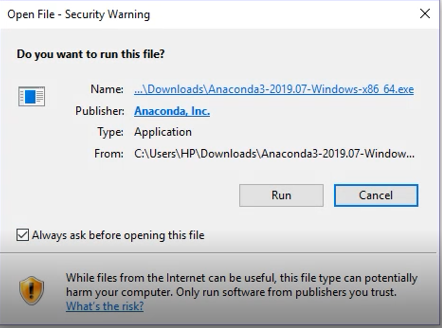
\includegraphics[scale=0.5]{figures/1}}
        \caption{Run Setup Anaconda}
		\label{langkah1}
\end{figure}

\item Tunggu sampai \textit{setup loading} selesai
\begin{figure}[H]
        \centerline{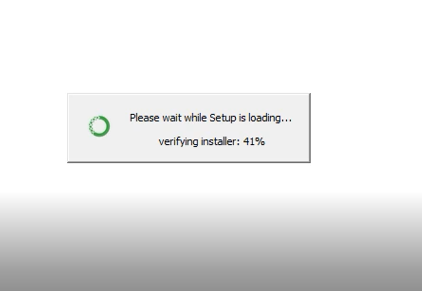
\includegraphics[scale=0.5]{figures/2}}
        \caption{Setup Loading}
		\label{langkah2}
\end{figure}


\item Jika \textit{setup loading} sudah selesai, maka selanjutnya klik \textit{next}
\begin{figure}[H]
        \centerline{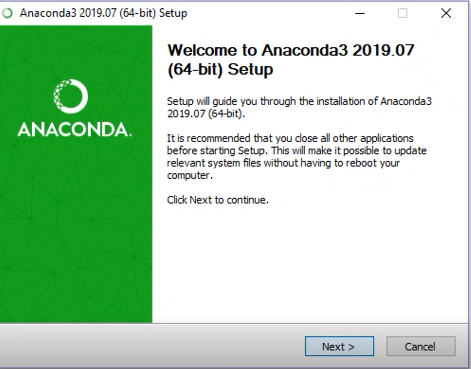
\includegraphics[scale=0.5]{figures/3}}
        \caption{Welcome to Anaconda Setup}
		\label{langkah2}
\end{figure}


\item Pada \textit{License Agreement} klik \textit{I Agree}
 gambar \textit{License Agreement}.

\begin{figure}[H]
    \centering
    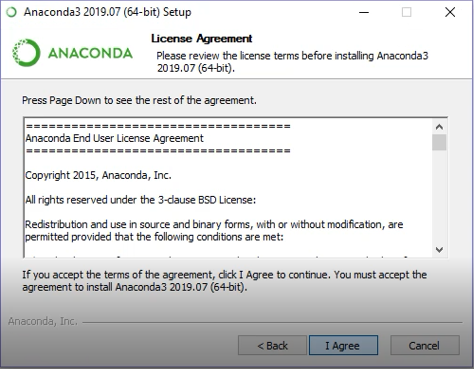
\includegraphics[scale=0.5]{figures/4}
    \caption{\textit{License Agreement}}
    \label{Figureanaconda3}
\end{figure}


\item Kemudian pilih \textit{Just Me(Recomended)} agar sesuai dengan komputer yang anda gunakan, kemudian klik \textit{next}
 gambar \textit{Just Me(recomended)}.

\begin{figure}[H]
    \centering
    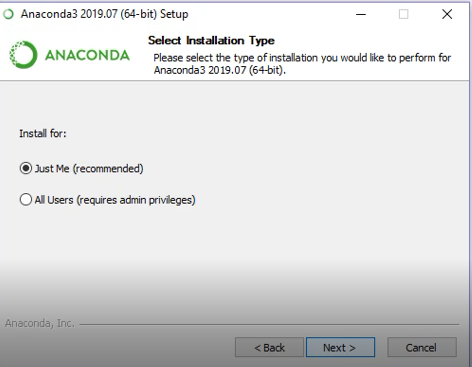
\includegraphics[scale=0.5]{figures/5}
    \caption{\textit{Just Me(recomended)}}
    \label{Figureanaconda4}
\end{figure}


\item Kemudian pilih lokasi tempat penyimpanan  \textit{installan anaconda}
 gambar \textit{Pilih lokasi}.

\begin{figure}[H]
    \centering
    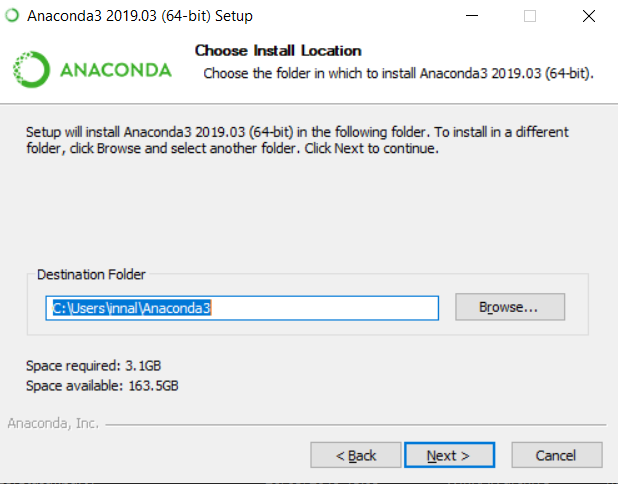
\includegraphics[scale=0.5]{figures/6}
    \caption{\textit{Pilih lokasi}}
    \label{Figureanaconda5}
\end{figure}

\item Kemudian centang \textit{Add Anaconda to my Path environtment variable}, agar saat \textit{menginstall selenium} langsung ke \textit{path anaconda} tidak ke aplikasi yang lain. Klik \textit{install}
 gambar \textit{Centang Anaconda to my PATH}.

\begin{figure}[H]
    \centering
    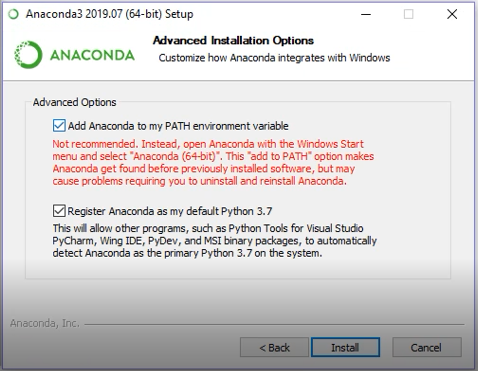
\includegraphics[scale=0.5]{figures/7}
    \caption{\textit{Centang Anaconda to my PATH}}
    \label{Figureanaconda6}
\end{figure}

\item Tunggu sampai proses \textit{installasi} selesai
 gambar \textit{Installation Complete}.

\begin{figure}[H]
    \centering
    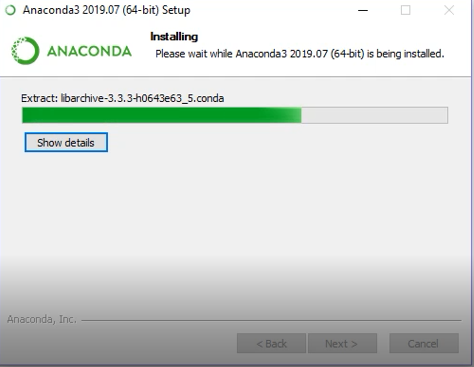
\includegraphics[scale=0.5]{figures/8}
    \caption{\textit{Installation Complete}}
    \label{Figureanaconda7}
\end{figure}

\item Apabila instalasi telah selesai klik \textit{next}
\begin{figure}[H]
    \centering
    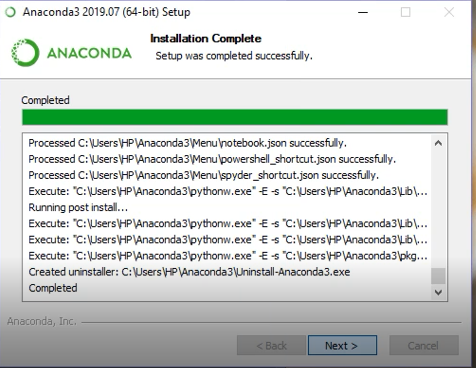
\includegraphics[scale=0.5]{figures/9}
    \caption{\textit{Installation Complete}}
    \label{Figureanaconda8}
\end{figure}

\item klik \textit{next}
\begin{figure}[H]
    \centering
    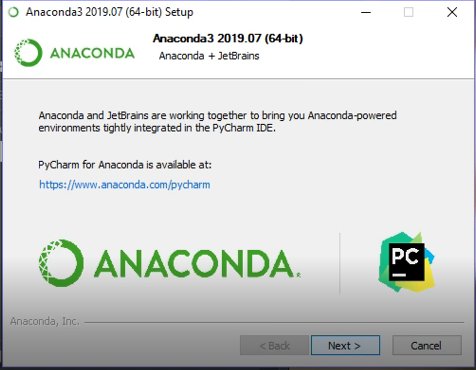
\includegraphics[scale=0.5]{figures/10}
    \caption{\textit{Anaconda+JetBrains}}
    \label{Figureanaconda70}
\end{figure}

\item Jika sudah klik \textit{finish}
 gambar \textit{Thanks fo install Anaconda}.

\begin{figure}[H]
    \centering
    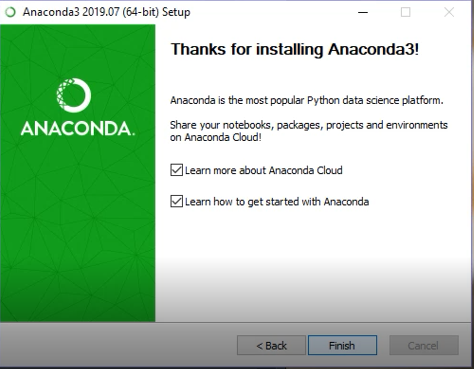
\includegraphics[scale=0.5]{figures/11}
    \caption{\textit{Thanks for install Anaconda}}
    \label{Figureanaconda70}
\end{figure}
\end{enumerate}

\subsection{Instalasi Pip}
\begin{enumerate}
\item buka anaconda promt
\item ketikkan conda install -c anaconda pip
\begin{figure}[H]
    \centering
    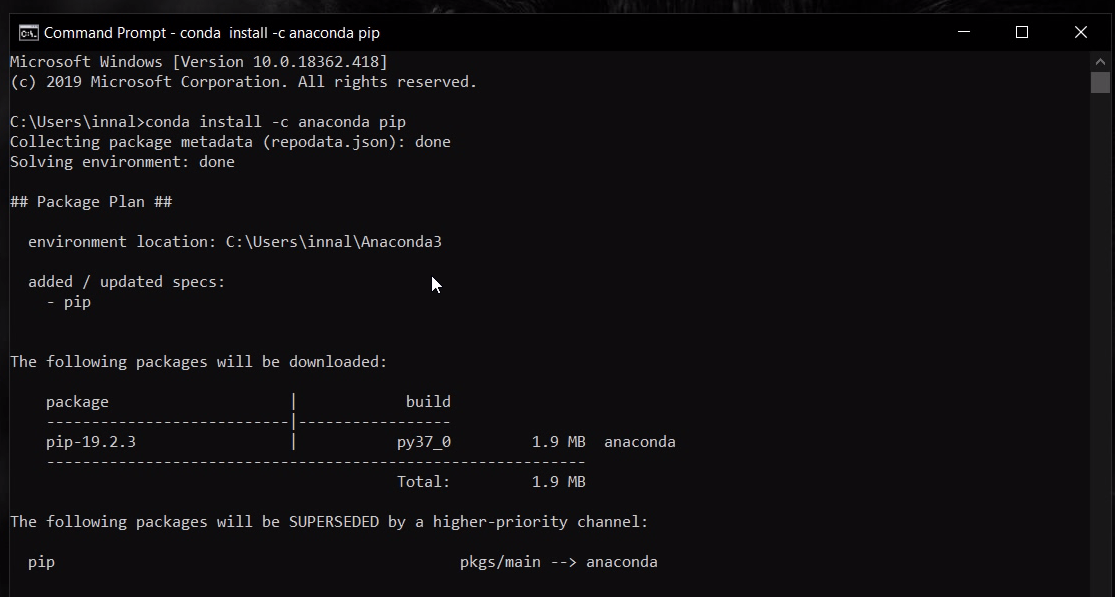
\includegraphics[scale=0.5]{figures/installpip}
    \caption{\textit{Install pip}}
    \label{Figureanaconda70}
\end{figure}
\item ketik y, lalu enter. Tunggu hingga proses instalasi selesai.
\begin{figure}[H]
    \centering
    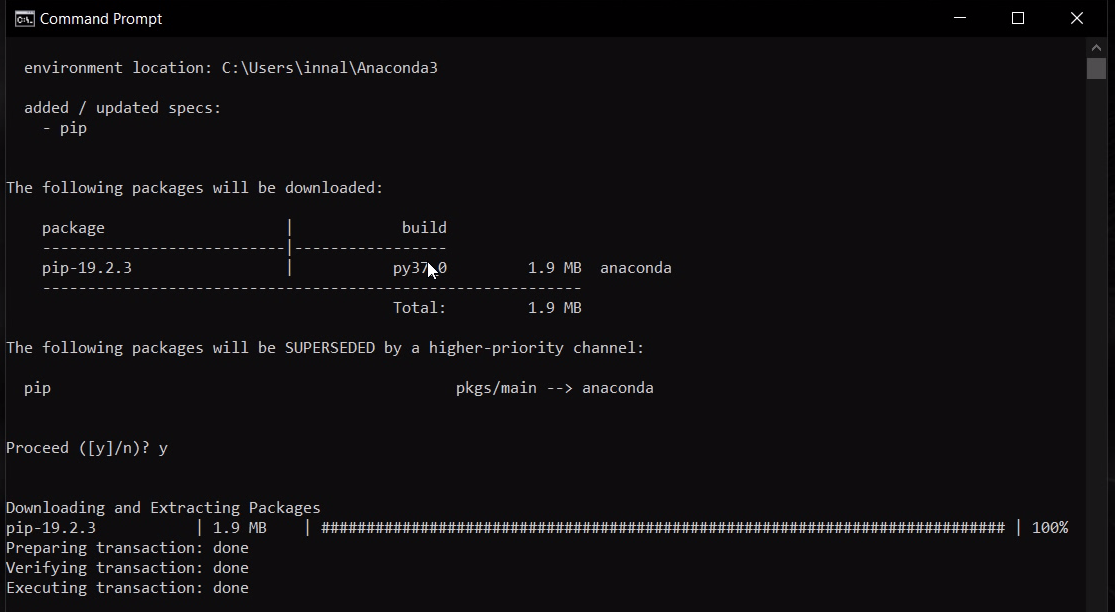
\includegraphics[scale=0.5]{figures/pipselesai}
    \caption{\textit{Install pip Selesai}}
    \label{Figureanaconda70}
\end{figure}
\item jika telah selesai, lakukan pengecekan versi pip dengan mengetikkan pip -V
\begin{figure}[H]
    \centering
    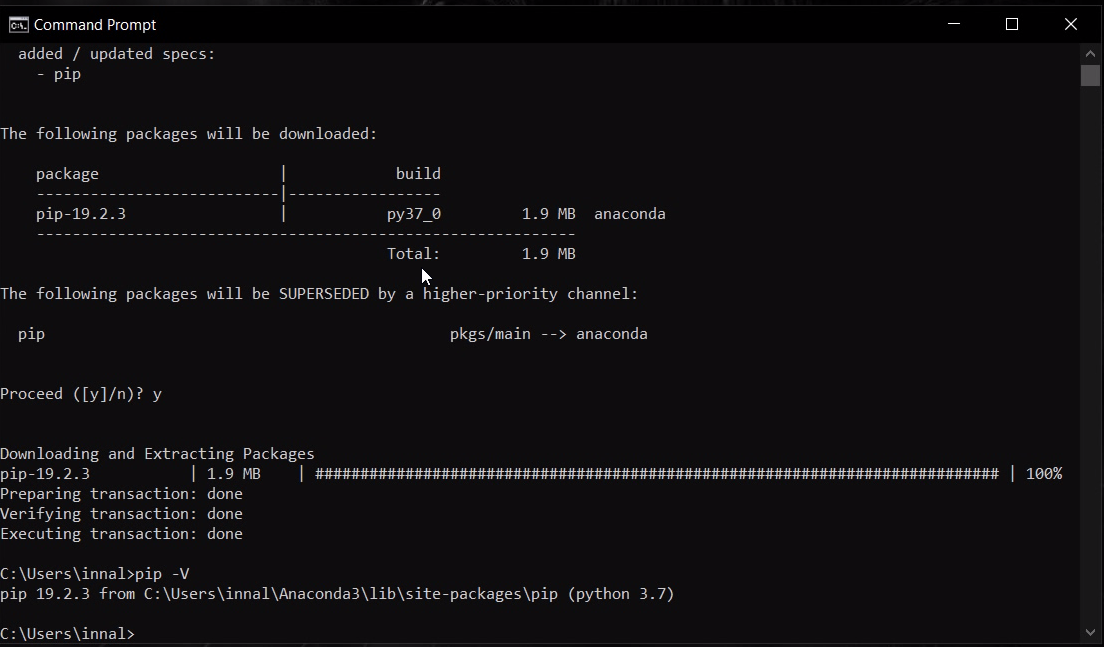
\includegraphics[scale=0.5]{figures/pipversion}
    \caption{\textit{Melihat Versi pip}}
    \label{Figureanaconda70}
\end{figure}

\end{enumerate}

\subsection{Setting Environment}
\begin{enumerate}
\item Buka file explorer
\item Klik kanan pada This pc, lalu pilih properties
\begin{figure}[H]
    \centering
    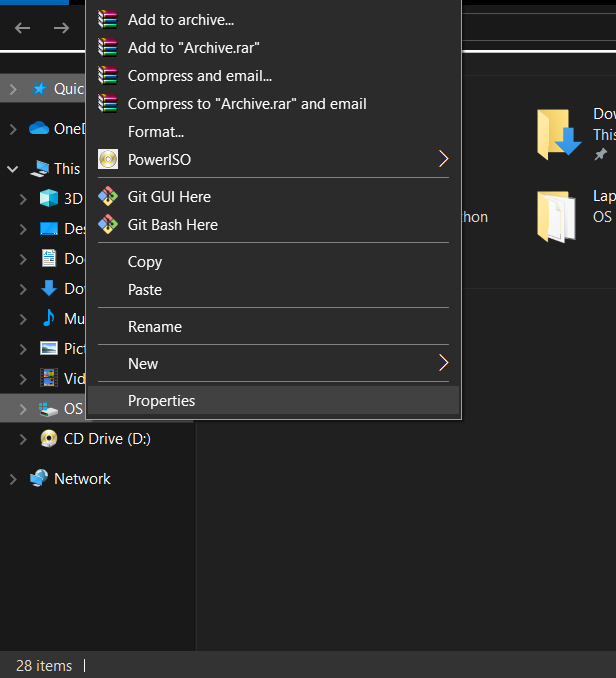
\includegraphics[scale=0.7]{figures/properties}
    \caption{\textit{Properties}}
    \label{Environment1}
\end{figure}
\item Pilih menu Advanced system settings
\begin{figure}[H]
    \centering
    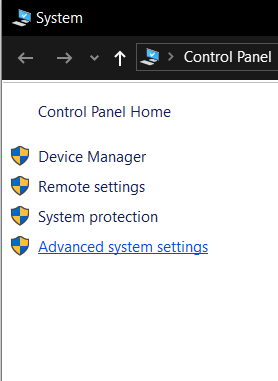
\includegraphics[scale=0.7]{figures/advanced}
    \caption{\textit{Advanced system settings}}
    \label{Environment2}
\end{figure}
\item Pilih Environment Variables
\begin{figure}[H]
    \centering
    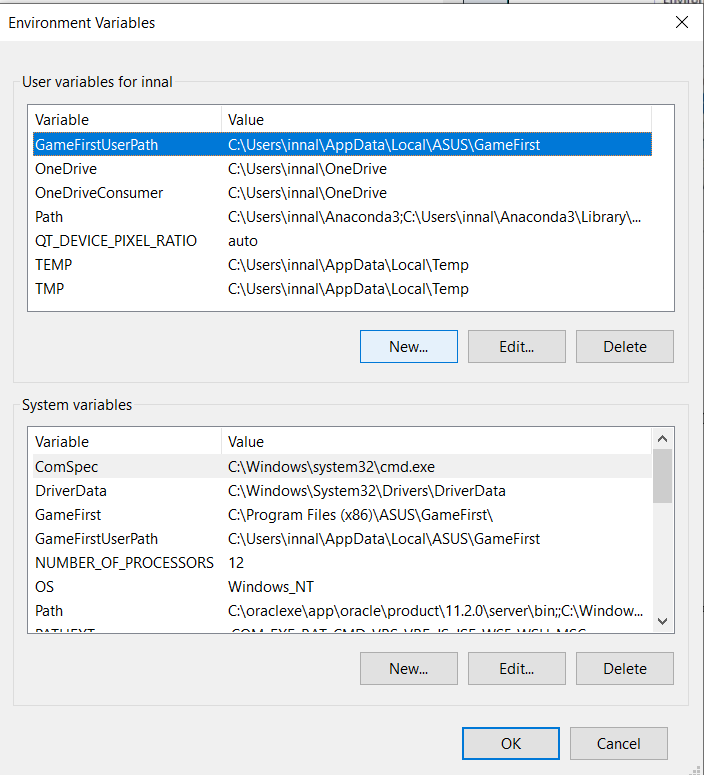
\includegraphics[scale=0.4]{figures/environment}
    \caption{\textit{Environment Variables}}
    \label{Environment3}
\end{figure}
\item Pilih Path
\begin{figure}[H]
    \centering
    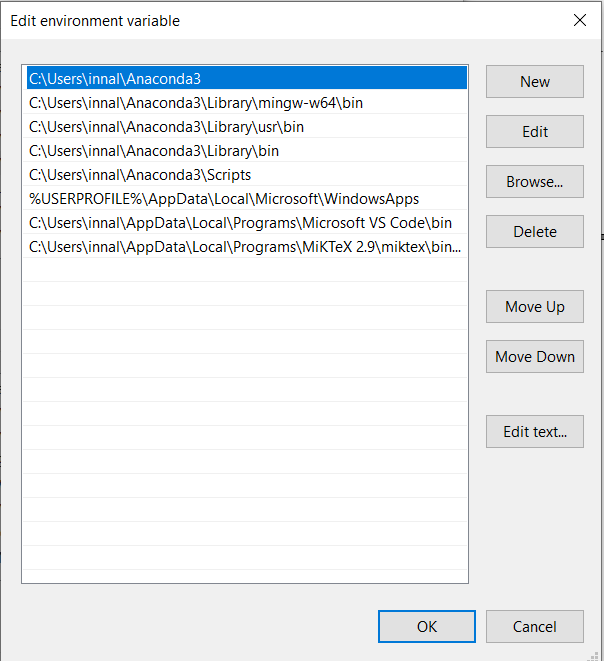
\includegraphics[scale=0.4]{figures/path}
    \caption{\textit{Path}}
    \label{Environment4}
\end{figure}
\item lalu pilih environment variable yang ingin ditambahkan, klik OK
\begin{figure}[H]
    \centering
    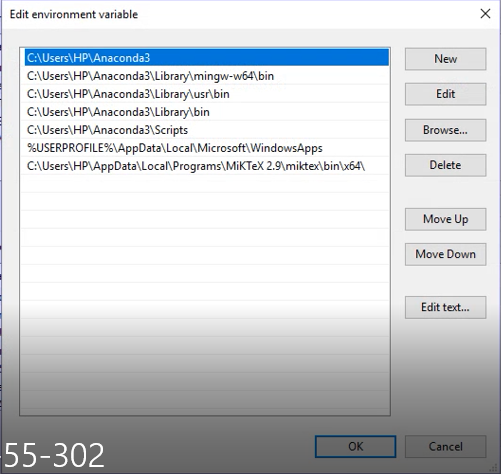
\includegraphics[scale=0.4]{figures/ok}
    \caption{\textit{Edit Environment Variable}}
    \label{Environment5}
\end{figure}
\end{enumerate}

\subsection{Command Line Interface/Interpreter}
\begin{enumerate}
\item Buka command prompt lalu ketikkan python
\item Buatlah perintah print, input, perkalian, dan pembagian
\item Bisa juga menjalankan file .py yang telah dibuat di IDE dengan cara python namafile.py, lalu klik enter
\begin{figure}[H]
    \centering
    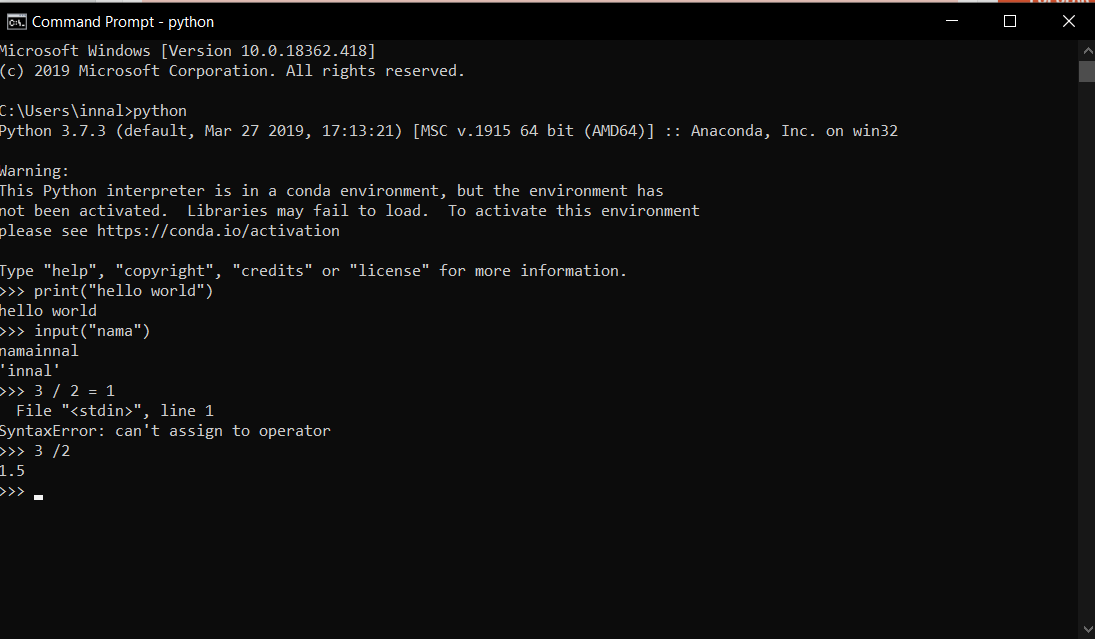
\includegraphics[scale=0.5]{figures/cli}
    \caption{\textit{CLI in Command Prompt}}
    \label{CLI}
\end{figure}
\end{enumerate}

\subsection{Update Anaconda dan Spyder}
\subsubsection{Anaconda} 
\begin{enumerate}
\item Ketikan conda install -c anaconda python di cmd
\begin{figure}[H]
    \centering
    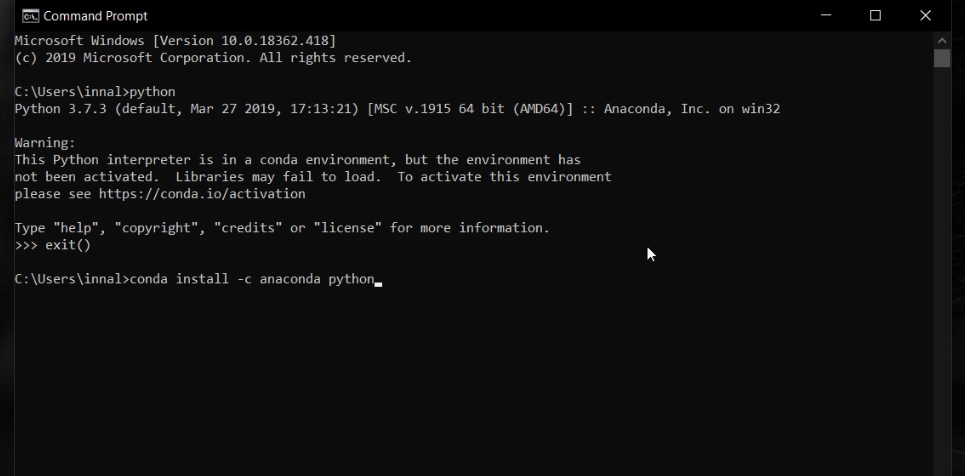
\includegraphics[scale=0.4]{figures/updatepython}
    \caption{\textit{Update python}}
    \label{Update Python}
\end{figure}
\item Ketikan y agar melanjutkan update
\begin{figure}[H]
    \centering
    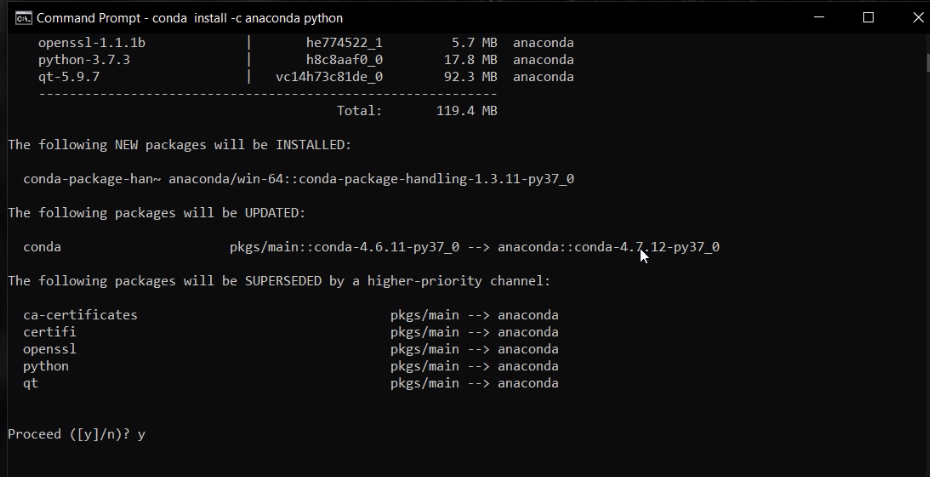
\includegraphics[scale=0.4]{figures/updatepythonyes}
    \caption{\textit{Update python yes}}
    \label{Update Python yes}
\end{figure}
\item Update selesai
\begin{figure}[H]
    \centering
    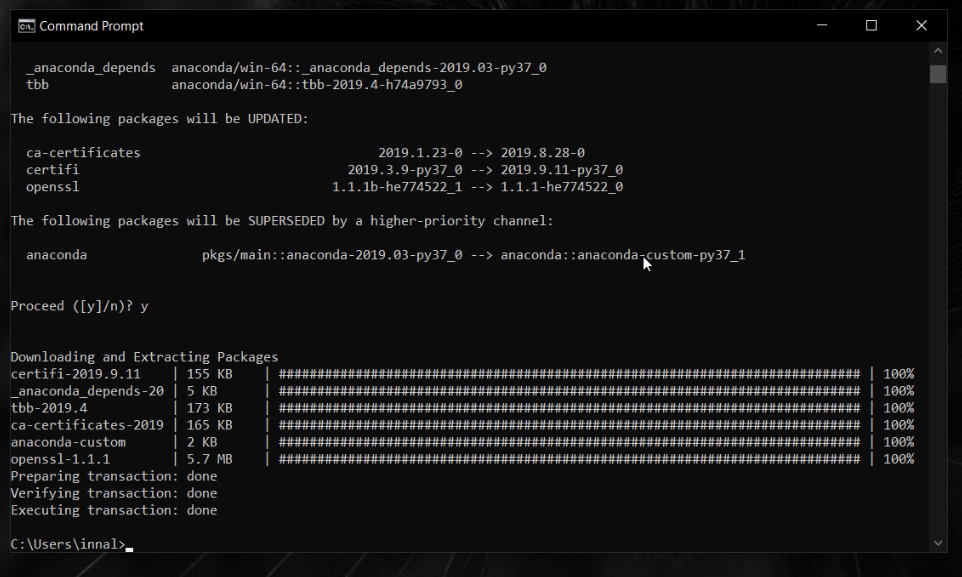
\includegraphics[scale=0.4]{figures/updatepythonselesai}
    \caption{\textit{Update python selesai}}
    \label{Update Python selesai}
\end{figure}
\end{enumerate}
\subsubsection{Spyder}
\begin{enumerate}
\item Ketikan conda install -c anaconda spyder di cmd
\begin{figure}[H]
    \centering
    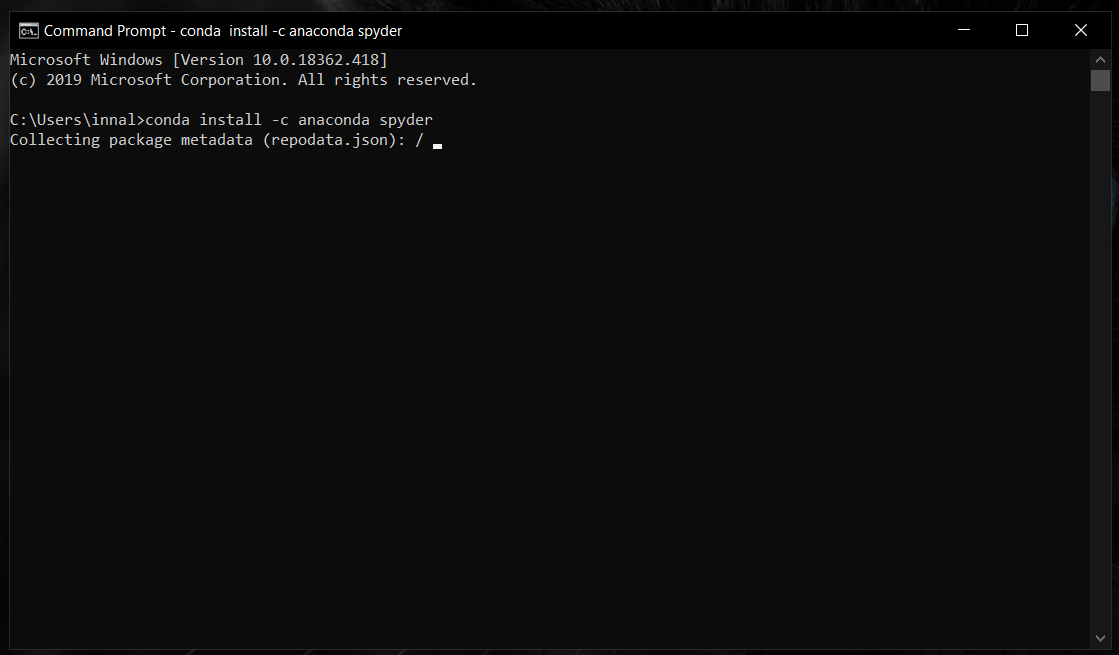
\includegraphics[scale=0.4]{figures/updatespyder}
    \caption{\textit{Update spyder}}
    \label{Update spyder selesai}
\end{figure}
\item update selesai
\begin{figure}[H]
    \centering
    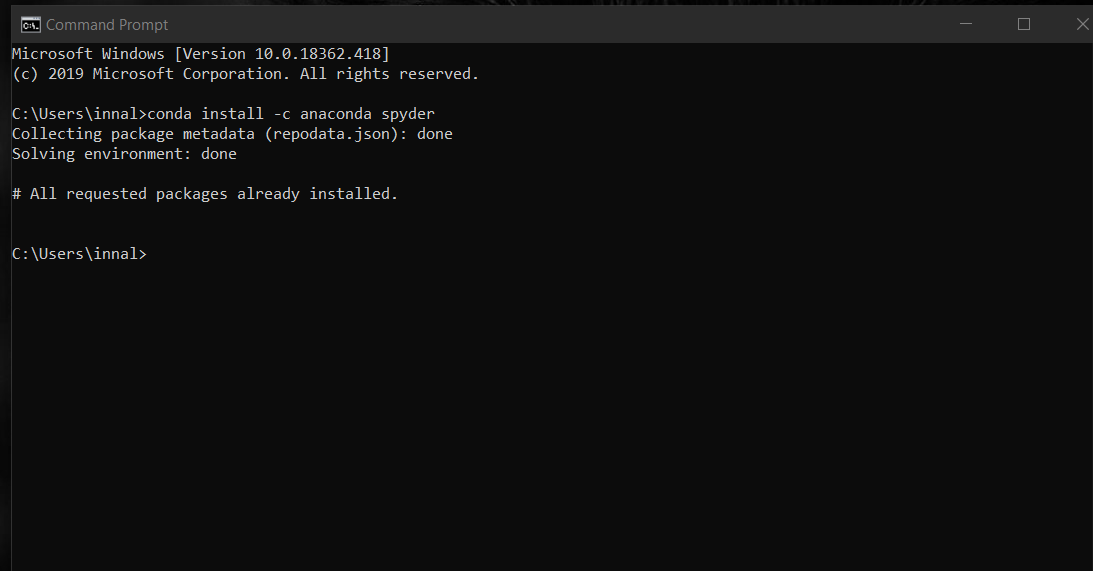
\includegraphics[scale=0.4]{figures/updatespyderselesai}
    \caption{\textit{Update spyder selesai}}
    \label{Update spyder selesai}
\end{figure}
\end{enumerate}

\subsection{Run Script Hello World di Spyder}
\begin{enumerate}
\item Buka anaconda navigator, lalu klik launch
\begin{figure}[H]
    \centering
    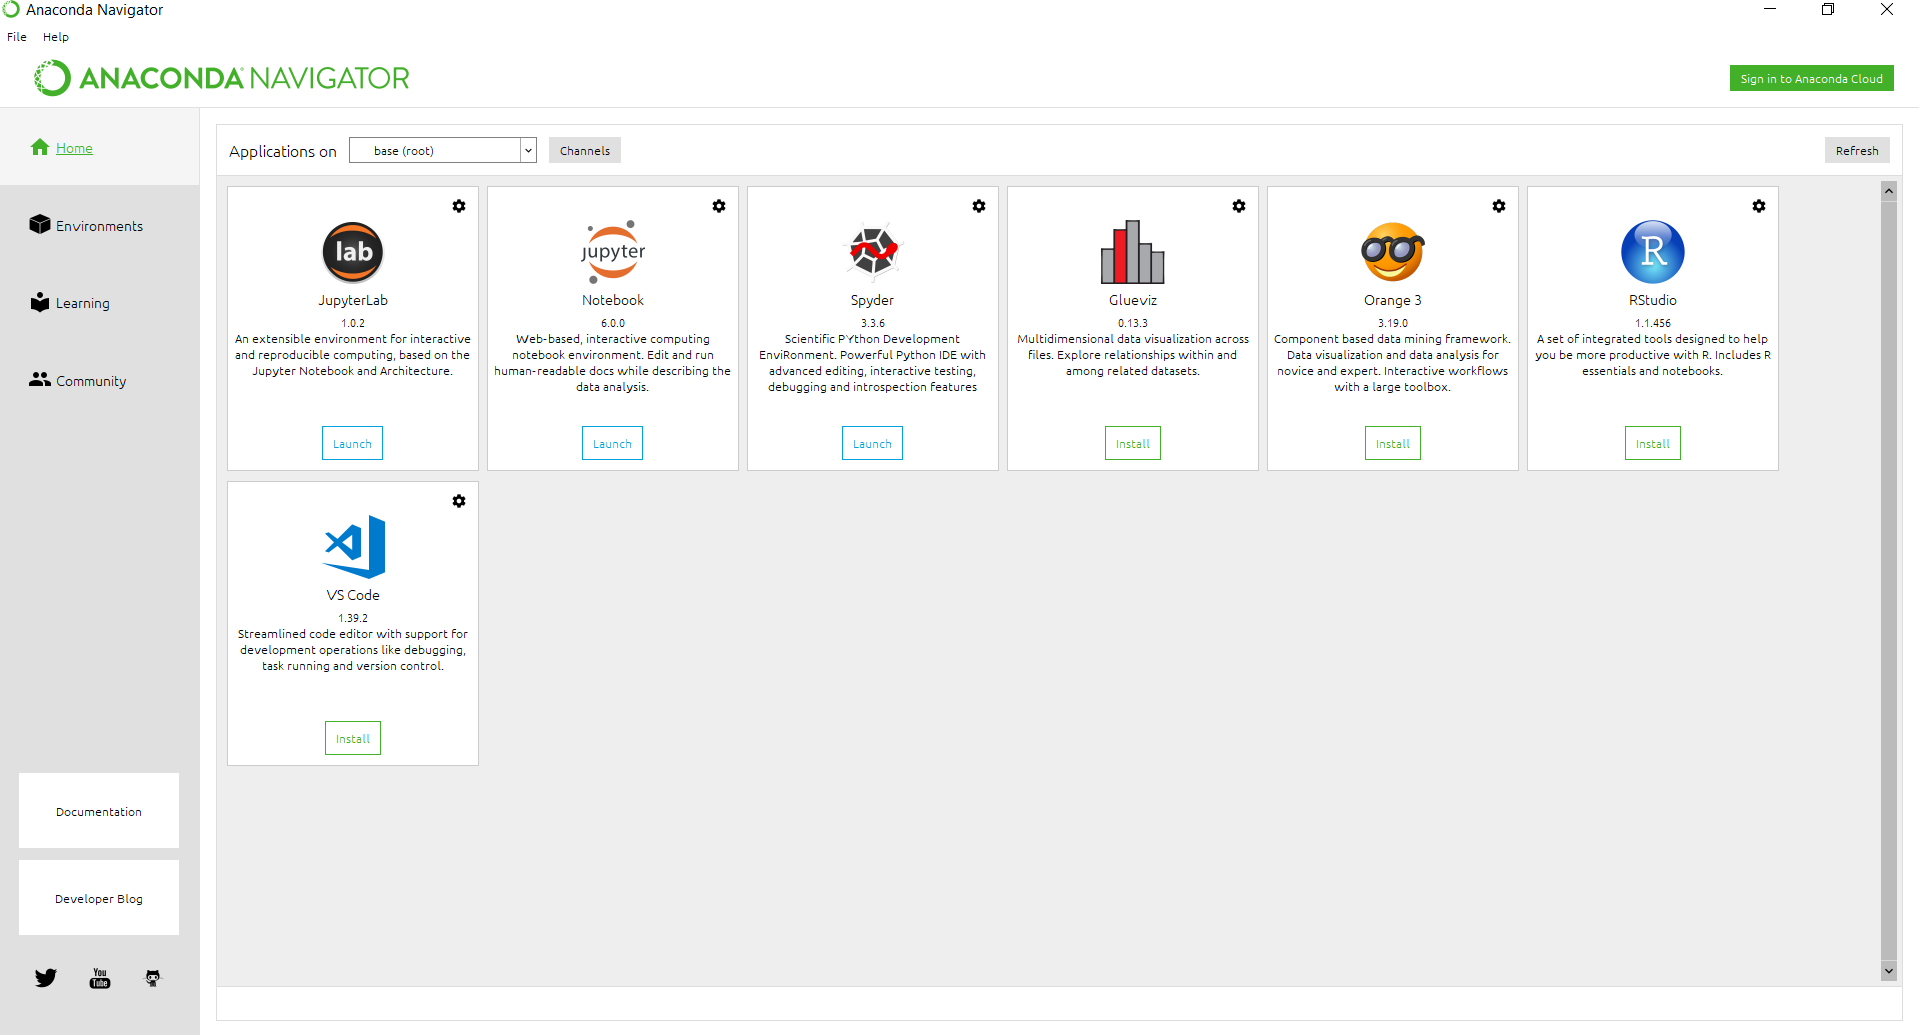
\includegraphics[scale=0.3]{figures/navigator}
    \caption{\textit{CLI in Command Prompt}}
    \label{Anaconda Navigator}
\end{figure}
\item ketikkan print("Hello World") dan run spyder
\begin{figure}[H]
    \centering
    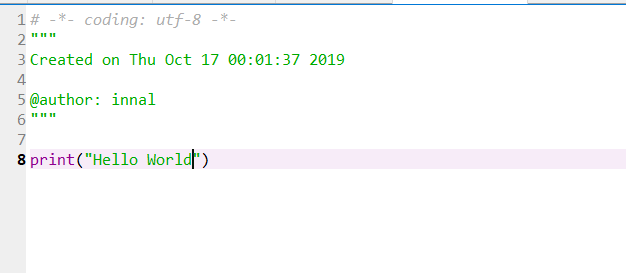
\includegraphics[scale=0.6]{figures/helloworld}
    \caption{\textit{Print Hello World}}
    \label{Print Hello World}
\end{figure}
\item hasilnya akan seperti ini
\begin{figure}[H]
    \centering
    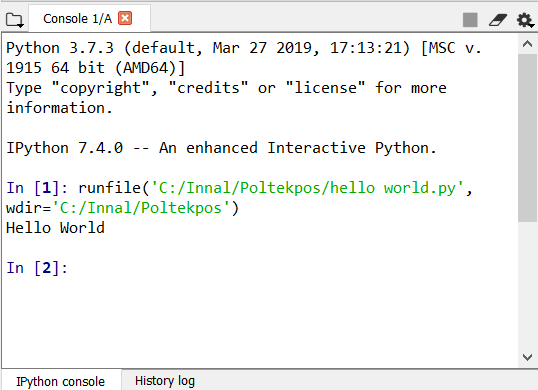
\includegraphics[scale=0.6]{figures/run}
    \caption{\textit{Hello World}}
    \label{Hello World}
\end{figure}
\end{enumerate}

\subsection{Automatic Login SIAP}
Buka Spyder lalu tuliskan script sebagai berikut.
\begin{verbatim}
from selenium.webdriver import Firefox
from selenium.webdriver.firefox.options import Options
from selenium.webdriver.common.desired_capabilities import DesiredCapabilities
from selenium.webdriver.firefox.firefox_binary import FirefoxBinary

print("Masukkan Npm Anda:")
npm = input()
print("Masukkan Password SIAP Anda:")
paswd = input('')

opsi = Options()

opsi.headless = False
binary = FirefoxBinary("C:\\Program Files\\Mozilla Firefox\\firefox.exe")
cap = DesiredCapabilities().FIREFOX
cap['marionette'] = True

browser=Firefox(executable_path='geckodriver.exe',
options=opsi,capabilities=cap,firefox_binary=binary)
browser.get('http://siap.poltekpos.ac.id/siap/besan.depan.php')

name = browser.find_element_by_name('user_name')
word = browser.find_element_by_name('user_pass')
login = browser.find_element_by_name('login')

name.send_keys(npm)
word.send_keys(paswd)
login.click()
\end{verbatim}
Kemudian save program dengan nama WA.py dan run program
\begin{figure}[H]
    \centering
    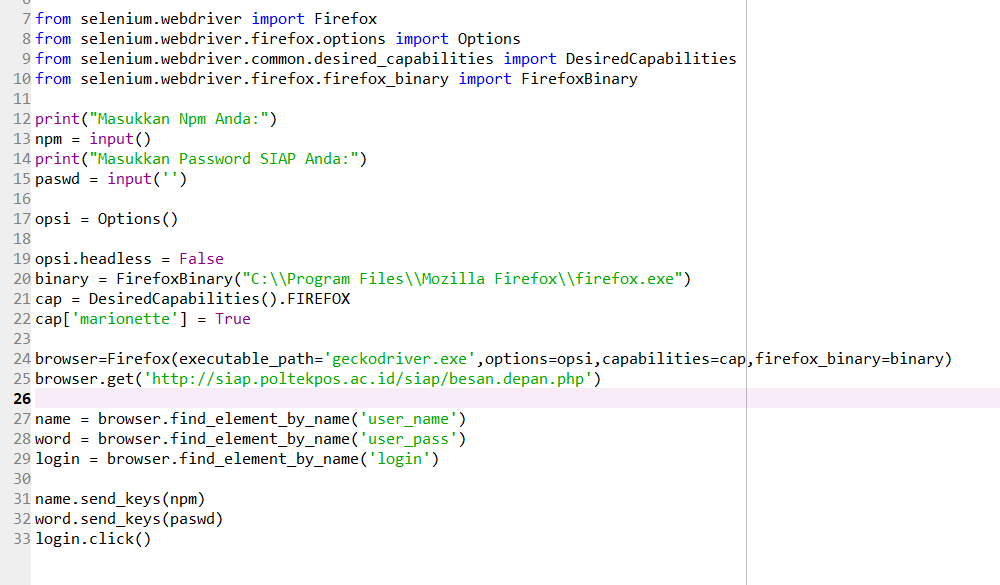
\includegraphics[scale=0.5]{figures/login}
    \caption{\textit{Automatic Login SIAP}}
    \label{Automatic1}
\end{figure}
Setelah di running maka kita akan diminta menginputkan npm dan Password akun SIAP
\begin{figure}[H]
    \centering
    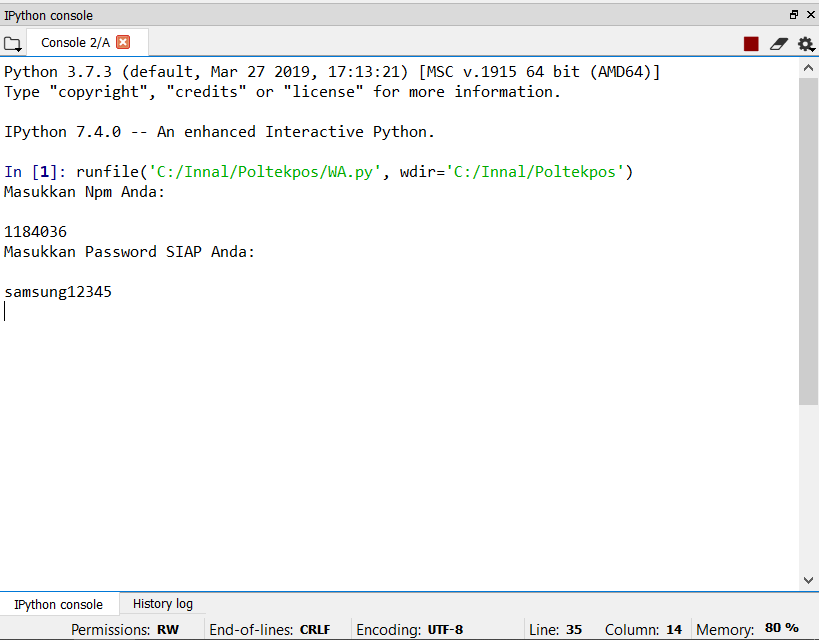
\includegraphics[scale=0.5]{figures/running}
    \caption{\textit{Hasil Running}}
    \label{Automatic2}
\end{figure}
Program selanjutnya akan membuka mozila secara otomatis dan mengetikkan npm serta password yang telah diinputkan oleh user dan kemudian mengklik login.
\begin{figure}[H]
    \centering
    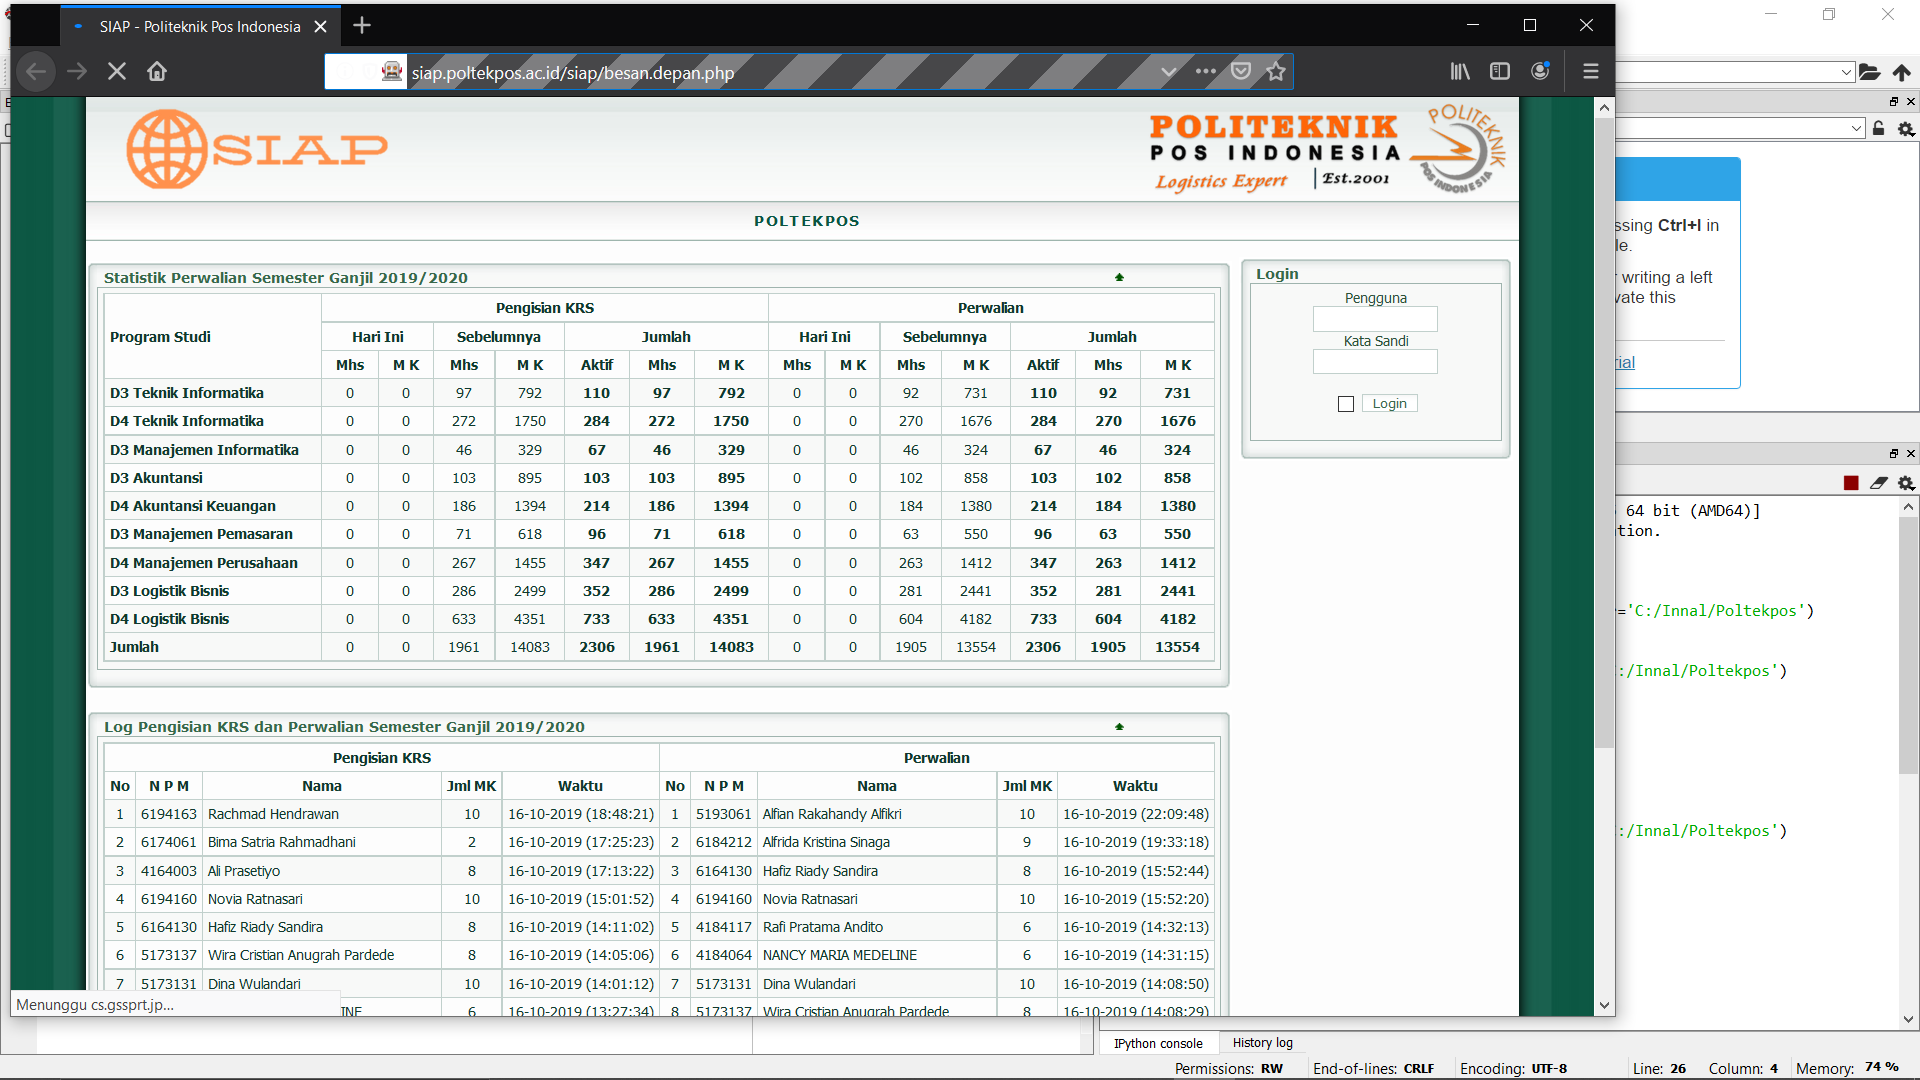
\includegraphics[scale=0.2]{figures/isi}
    \caption{\textit{Automatic Input dan Login}}
    \label{Automatic3}
\end{figure}
Login selesai
\begin{figure}[H]
    \centering
    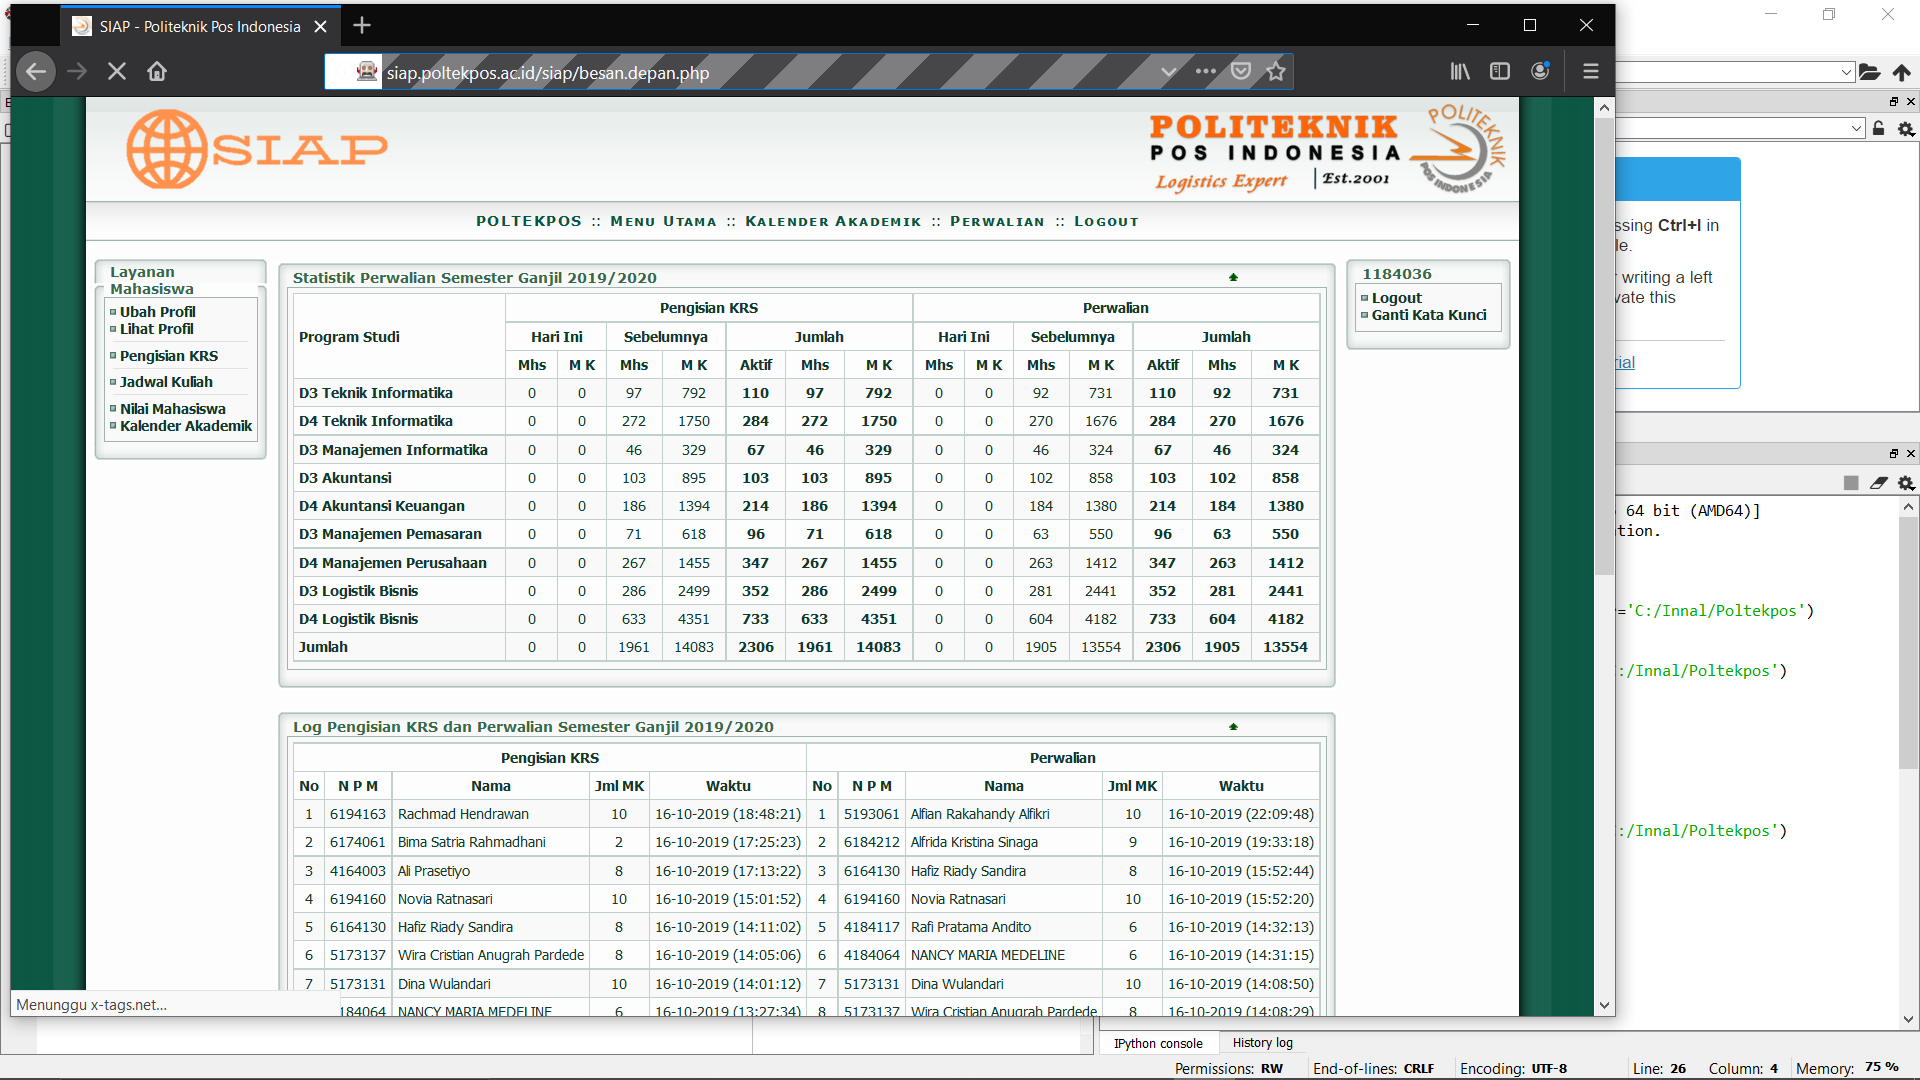
\includegraphics[scale=0.2]{figures/loginselesai}
    \caption{\textit{Automatic Input dan Login Selesai}}
    \label{Automatic4}
\end{figure}

\subsection{Pemakaian Variable Explorer}
Variable explorer akan secara otomatis terisi ketika kita menbuat sebuah variable, pada variable explorer kita bisa melihat nama variable, tipe data, length, dan value dari variable yang kita buat tersebut.
\begin{figure}[H]
    \centering
    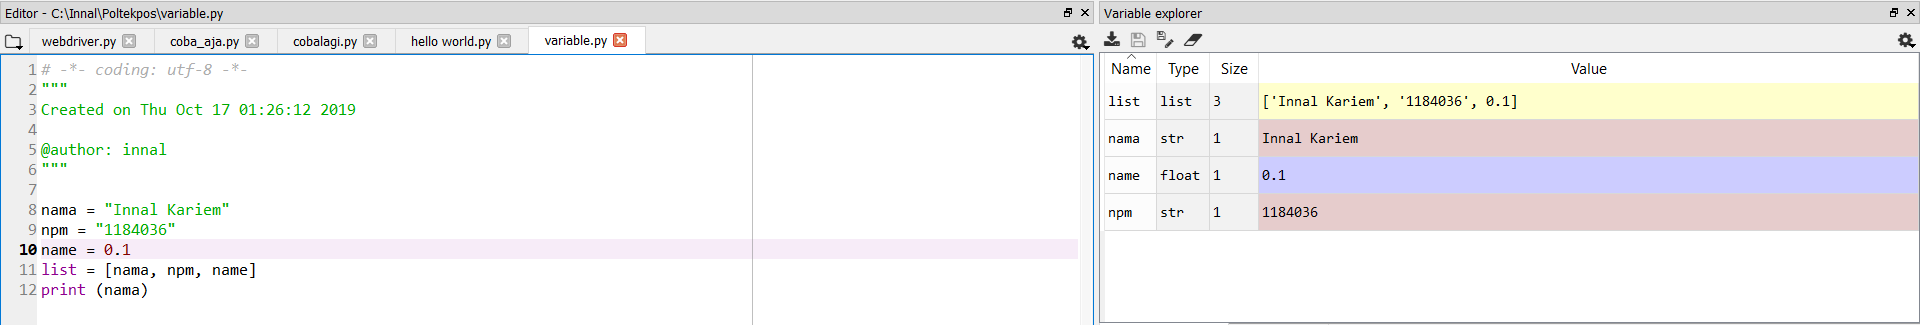
\includegraphics[scale=0.3]{figures/variable}
    \caption{\textit{Variable Explorer}}
    \label{Variable Explorer}
\end{figure}

\section{Indentasi}
\subsection{Penjelasan Indentasi}
Identasi, bagian code paragraf yang posisinya menjorok ke dalam pada baris-baris paragraf code. untuk mengatur indentasi dapat menggunakan tab atau spasi. Identasi biasa digunakan oleh bahasa pemrograman python sebagai pengganti briket ({}) untuk membuka dan menutup fungsi. Error indentasi dapat terjadi apabila syntax tidak menggunakan tab atau space.
Contoh yang benar (menggunakan tab/spasi sebagai indentasi):
\begin{verbatim}
# percabangan if
if username == 'crot':
    print("Selamat Datang ganteng")
    print("Silahkan ambil air wudhu")

# blok percabangan for
for i in range(10):
    print i
\end{verbatim}
Contoh yang salah (tidak menggunakan tab/spasi):
\begin{verbatim}
# percabangan if
if username == 'crot':
print("Selamat Datang ganteng")
print("Silahkan ambil air wudhu")

# percabangan for
for i in range(10):
print i
\end{verbatim}

\subsection{Jenis-Jenis Error Indentasi}
IndentationError: unexpected indent. Error diatas terjadi apabila syntax kekurangan tab atau spasi.
\begin{figure}[H]
    \centering
    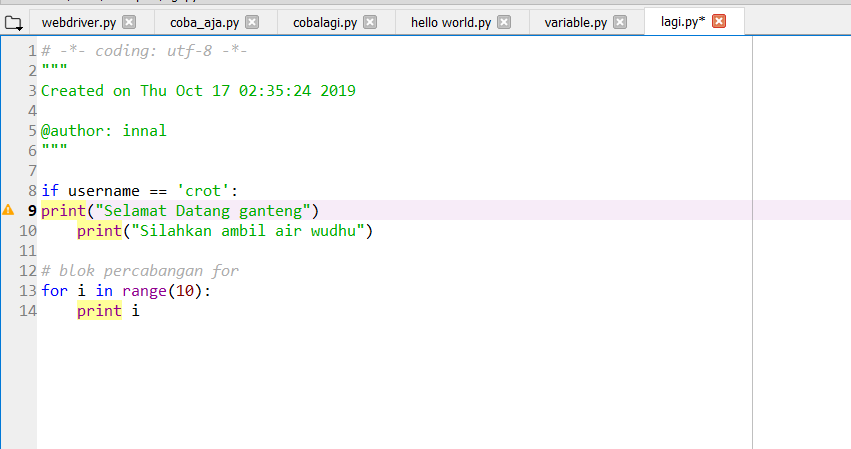
\includegraphics[scale=0.2]{figures/indentasi}
    \caption{\textit{Indentasi}}
    \label{Indentasi}
\end{figure}
Apabila di running akan memunculkan error sebagai berikut.
\begin{figure}[H]
    \centering
    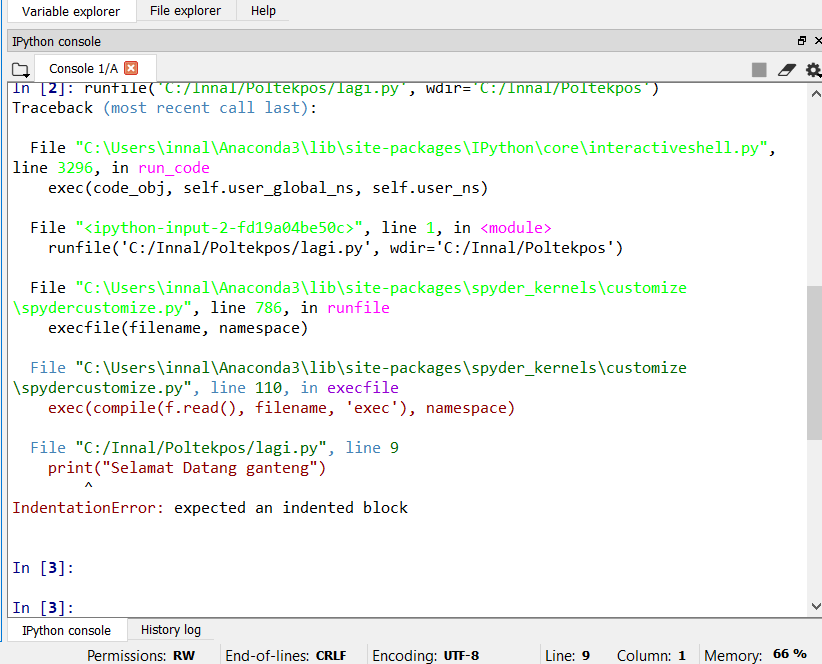
\includegraphics[scale=0.4]{figures/errorindentasi}
    \caption{\textit{Error Indentasi}}
    \label{Error Indentasi}
\end{figure}

\subsection{Cara Membaca Error}
Jika terjadi error maka cari di console line berapa yang error, pada gambar berikut terdapat error indentasi pada line 9.
\begin{figure}[H]
    \centering
    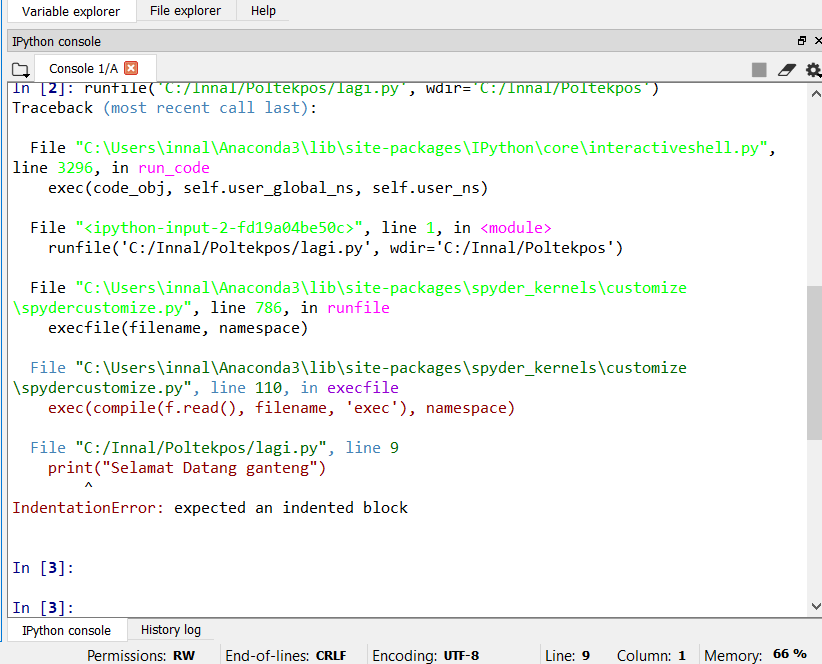
\includegraphics[scale=0.4]{figures/errorindentasi}
    \caption{\textit{Error}}
    \label{Error}
\end{figure}

\subsection{Cara Menangani Error}
Untuk Menangani error indentasi dapat dilakukan dengan cara menambahkan tab atau space pada line yang error.
Berikut syntax yang error.
\begin{figure}[H]
    \centering
    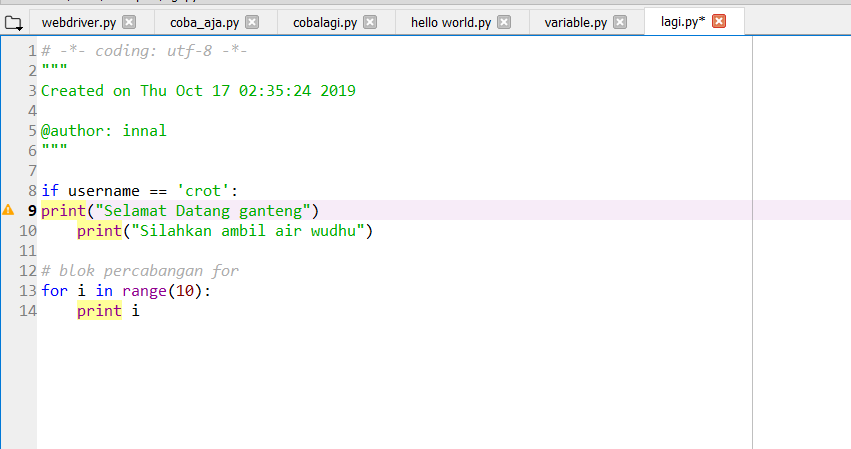
\includegraphics[scale=0.4]{figures/indentasi}
    \caption{\textit{Syntax Error}}
    \label{Syntax Error}
\end{figure}
Berikut syntax yang tidak error menggunakan tab/spasi (indentasi).
\begin{figure}[H]
    \centering
    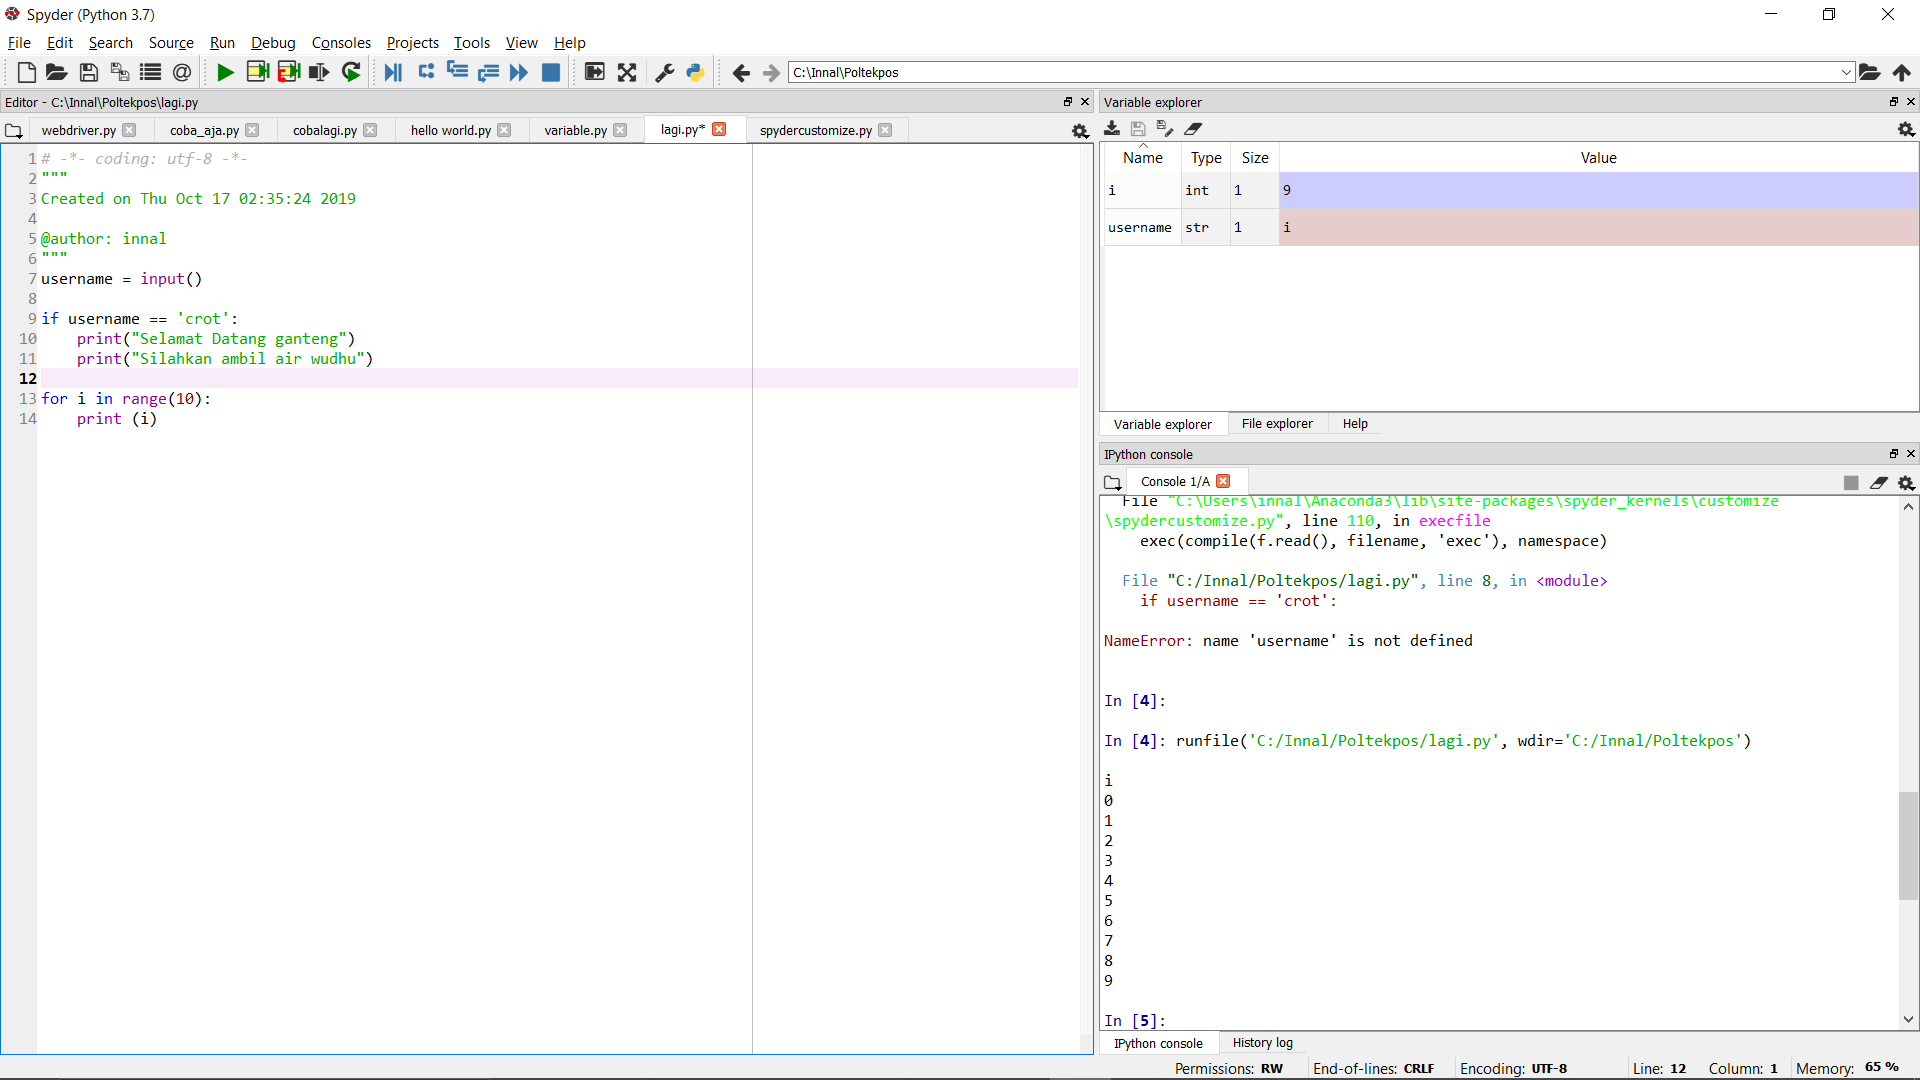
\includegraphics[scale=0.2]{figures/indentasicoy}
    \caption{\textit{Syntax yang Telah Diperbaiki}}
    \label{Syntax Error}
\end{figure}